\documentclass{standalone}
\usepackage{tikz} % tikz
\usepackage{standalone} % tikz figures are often in standalone
\usepackage{amsfonts} % mathbb etc
\usepackage{amsmath} % crucial package
\usepackage{amsthm} % ams-style theorems
\usepackage{bm} % bold math symbols
\usepackage{xcolor} % more colors
\usepackage[T1]{fontenc} % modern encoding, better than OT1, the default

\newtheorem{definition-fr}{Définition}
\newtheorem{example-fr}{Exemple}
\newtheorem{theorem-fr}{Théorème}
\newtheorem{proposition-fr}{Proposition}
\newtheorem{lemma-fr}{Lemme}
\newtheorem{remark-fr}{Remarque}
\newtheorem{definition}{Definition}
\newtheorem{lemma}{Lemma}
\newtheorem{proposition}{Proposition}
\newtheorem{remark}{Remark}

\usetikzlibrary{decorations.pathmorphing} % for snake, zigzag...
\usetikzlibrary{positioning} % for the "below of=1cm" type of options
\usetikzlibrary{intersections} % e.g. for pyramid
\usetikzlibrary{calc} % for computing node coordinates from others
\usetikzlibrary{overlay-beamer-styles} % when \pause glitches in tikz beamer
\usetikzlibrary{arrows} % arrows
\usetikzlibrary{external} % only compile the figure the first time
\tikzexternalize[only named=true, prefix=tikz-cache/]
\immediate\write18{mkdir -p latex-build/tikz-cache}

% used to pass "scale=XX" as includetikz option
\pgfkeys{
  /tikzoptions/.is family, % Namespace
  /tikzoptions/.cd, % Namespace
  scale/.store in=\scale, % Store the value of 'scale'
}

% usage: \includetikz[scale=XX]{fig}, fetches from my local database
\newcommand{\includetikz}[2][scale=1]{
  \bgroup
  \pgfkeys{/tikzoptions,#1} % currently only accepts 'scale' (april 9 2025)
  \tikzsetnextfilename{#2}
  \include{tex-macros/tikz-figures/#2}% Include the standalone TikZ file
  \egroup
}

% usage: \inputtikz[scale=XX]{fig}, fetches from my local database
\newcommand{\inputtikz}[2][scale=1]{
  \bgroup
  \pgfkeys{/tikzoptions,#1} % currently only accepts 'scale' (april 9 2025)
  \tikzsetnextfilename{#2}
  \input{tex-macros/tikz-figures/#2}% Include the standalone TikZ file
  \egroup
}


\newcommand{\bigOt}{\widetilde{\mathcal{O}}}
\newcommand{\bigO}{\mathcal{O}}

\definecolor{mypurp}{HTML}{8f0c97}
\definecolor{myred}{HTML}{9f103b}
\definecolor{myor}{HTML}{ae3011}
\definecolor{mydarkor1}{HTML}{96240f}
\definecolor{mydarkor2}{HTML}{7f180c}
\definecolor{mylb1}{HTML}{00557e}
\definecolor{mylb2}{HTML}{013157}
\definecolor{mybl1}{HTML}{0d08a9}
\definecolor{mybl2}{HTML}{04037f}
\definecolor{mygr1}{HTML}{097e3e}
\definecolor{mygr2}{HTML}{025520}
\definecolor{myyellow}{HTML}{FFD700}



\makeatletter
\@ifundefined{scale}{
  \def\scale{1}
}
\makeatother


\begin{document}
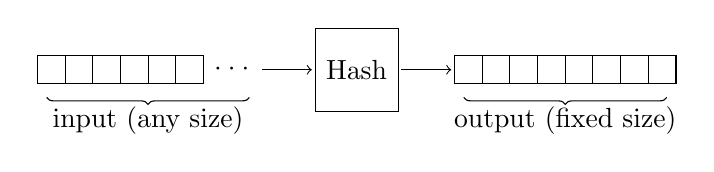
\begin{tikzpicture}
  \def\boxw{1em}
  \def\boxh{1em}
  \def\hboxw{3em}
  \def\hboxh{\hboxw}
  \def\dotsdist{.5em}
  \def\arrowlength{2em}
  \def\arrowmargin{.1em}
  \def\bracedist{1em}
  \newcounter{inputnb}
  \setcounter{inputnb}{6}
  \edef\in{\arabic{inputnb}}
  \newcounter{dotsnb}
  \setcounter{dotsnb}{3}
  \edef\dn{\arabic{dotsnb}}
  \newcounter{outputnb}
  \setcounter{outputnb}{8}
  \edef\out{\arabic{outputnb}}

  \tikzstyle{datarec} = [draw, rectangle, minimum width=\boxw, minimum height=\boxh]
  \tikzstyle{hashrec} = [draw, rectangle, minimum width=\hboxw, minimum height=\hboxh]
  \tikzstyle{myarrow} = [->, shorten >= \arrowmargin, shorten <= \arrowmargin]

  \foreach \i in {1,...,\in} {
    \node[datarec] (in\i) at (\i*\boxw,0) {};
  }
  \foreach \i in {1,...,\dn} {
    \node (dn\i) at ($(in\in.east) + (\i*\dotsdist,0)$) {$\cdot$};
  }
  \node[hashrec, anchor=west] (hash) at ($(dn\dn.east) + (\arrowlength,0)$) {Hash};
  \draw[myarrow] (dn\dn) -- (hash);

  \foreach \i in {1,...,\out} {
    \node[datarec, anchor=west] (out\i) at ($(hash.east) + ({\arrowlength + (\i-1)*\boxw},0)$) {};
  }
  \draw[myarrow] (hash) -- (out1);

  \node[yshift=-\bracedist] (brace1l) at (in1.west) {};
  \node[yshift=-\bracedist] (brace1r) at (dn\dn.east) {};
  \draw[decorate, decoration={brace}] (brace1r) -- node[below] {input (any size)} (brace1l);

  \node[yshift=-\bracedist] (brace2l) at (out1.west) {};
  \node[yshift=-\bracedist] (brace2r) at (out\out.east) {};
  \draw[decorate, decoration={brace}] (brace2r) -- node[below] {output (fixed size)} (brace2l);
\end{tikzpicture}
\end{document}
